\section{Introduction}

Welcome to this Practical Abhidhamma Course. This first talk provides context; it will introduce the Abhidhamma as part of the Buddhist canon and will discuss its historical development.

During this talk you should have the \textit{Satipaṭṭhāna} Sutta\footnote{\url{http://en.wikipedia.org/wiki/Satipatthana_Sutta}} printout and Handout 1 in front of you. Please use the version of the \textit{Satipaṭṭhāna} Sutta provided\footnote{The original (without paragraph numbers) can be downloaded from \url{http://www.accesstoinsight.org/tipitaka/mn/mn.010.nysa.html}. I chose this translation of the \textit{Satipaṭṭhāna} Sutta because of the number of end-notes.} as I will be referencing the paragraph numbers from this version.

Handout 1 has three diagrams. The top diagram shows the “Structure of the Buddhist Canon,” the middle diagram shows “Topics in the Suttas and Abhidhamma,” and the bottom diagram is a “Timeline.”

\subsection*{Structure of the Buddhist canon}

Let’s start by looking at the top diagram showing the structure of the Buddhist canon.

\begin{figure}[H]
\centering
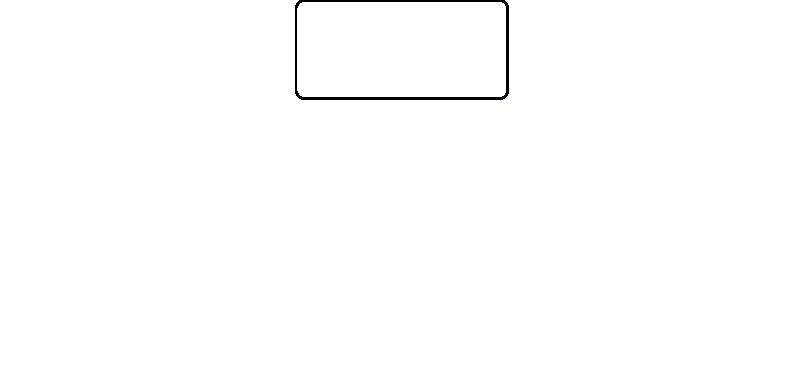
\includegraphics[width=0.6\linewidth]{./Diagrams/Tipitaka}
\caption{The Pāḷi \textit{Tipiṭaka} consists of three collections.}
\label{fig:Tipitaka}
\end{figure}

\textit{Tipiṭaka}\footnote{\url{http://en.wikipedia.org/wiki/Tipitaka}} is a Pāḷi word. In Pāḷi, \textit{Ti} means three and \textit{Piṭaka} means basket, so \textit{Tipiṭaka} is literally “three baskets” meaning “three collections.” The first collection is the Vinaya – the rules for monks and nuns. The second collection is the Suttas – the spoken discourses given by the Buddha and his disciples using conventional language. The third collection is the Abhidhamma – providing a detailed framework covering all the teachings. \textit{Abhi} is a Pāḷi prefix meaning “higher” \footnote{In “The Expositor” (\textit{Atthasālinī}) page 3, Buddhaghosa explains that the prefix “\textit{Abhi}” also indicates that the Abhidhamma “exceeds and is distinguished from the Dhamma (the Suttas).”} and so Abhidhamma literally means higher teachings.

Let me help you to visualize the size of the \textit{Tipiṭaka}.\footnote{In the world’s largest book (\url{http://en.wikipedia.org/wiki/World’s_largest_book}), the entire \textit{Tipiṭaka} is written in Pāḷi using Burmese script on the front and back of 729 marble slabs (total of 1458 “pages”); 222 “pages” of Vinaya, 820 “pages” of Suttas and 416 “pages” of Abhidhamma.} The printed \textit{Tipiṭaka} fills a bookshelf one metre in length. The Suttas make up about half of the \textit{Tipiṭaka}, the Abhidhamma makes up about one third of the \textit{Tipiṭaka} and the Vinaya makes up about one sixth of the \textit{Tipiṭaka}.

\pagebreak

Over the past 60 years, 11 monks in Myanmar have memorized the entire \textit{Tipiṭaka}.\footnote{These monks are given the title “\textit{Tipiṭaka dhara}”: \url {http://www.myanmarnet.net/nibbana/tipitaka/tpdkdhra.htm}} The first of these monks\footnote{\url{http://en.wikipedia.org/wiki/Mingun_Sayadaw}} got into the Guinness Book of Records for reciting 16,000 pages of the \textit{Tipiṭaka}. Amazing! I have become so dependent on technology that sometimes I can’t even remember my wife’s phone number!

\subsection*{Vinaya}

The first part of the \textit{Tipiṭaka} is the Vinaya.\footnote{\url{http://en.wikipedia.org/wiki/Vinaya_Pitaka}} In the Vinaya, the Buddha used his authority to lay down rules and procedures for monks and nuns. The community of monks and nuns, the Sangha,\footnote{\url{http://en.wikipedia.org/wiki/Sangha}} would not have survived for 2,600 years without a body of rules and procedures to keep them strong.\footnote{The Buddha excelled not only as a teacher (in the Suttas), but also as an administrator (in the Vinaya).}

The Vinaya includes 227 major rules for monks and 311 major rules for nuns.\footnote{This group of major rules is called the \textit{Pāṭimokkha}, (\url{http://en.wikipedia.org/wiki/Patimokkha}). The Sangha recite the \textit{Pāṭimokkha} twice a month during the \textit{Uposatha} ceremony (\url{http://www.accesstoinsight.org/ptf/dhamma/sila/uposatha.html}).} There are also hundreds of supplementary rules. There are a different number of rules for monks and for nuns because rules were established only when incidents were brought to the attention of the Buddha.\footnote{The Buddha was pragmatic; he modified rules and procedures as circumstances changed.} Each individual rule focuses on harmonious interactions between monastics\footnote{This story from the Commentary stresses the importance of harmonious interactions between monastics: \url{http://www.tipitaka.net/tipitaka/dhp/verseload.php?verse=006}} and blameless interactions with laypeople.\footnote{According to the Vinaya, Volume 1, page 37--38, the Vinaya rules are meant to: 1) Protect the Community 2) Insure the Community’s comfort 3) Ward off ill-meaning people 4) Help well-behaved monks and nuns 5) Destroy present defilements 6) Prevent future defilements 7) Benefit non-followers 8) Increase the number of followers 9) Establish the Discipline 10) Observe the rules of restraint.} As a complete set, the rules create an environment that is conducive to spiritual development.

The Vinaya is like a legal text. It describes the origin of each rule and gives many examples of how each rule is to be applied, what constitutes an offence and what does not; information that helps the Sangha to interpret the rules properly.\footnote{This material is found in Volume 1 of the Vinaya (\textit{Sutta Vibhaṅga}).}

\subsection*{Suttas}

Now let’s talk a bit about the Suttas,\footnote{\url{http://en.wikipedia.org/wiki/Sutta_Pitaka}} the discourses given by the Buddha and his disciples. The Sutta \textit{Piṭaka} contains more than 10,000 Suttas\footnote{The Dīgha Nikāya has 34 Suttas, the Majjhima Nikāya has 152 Suttas, the Saṃyutta Nikāya has 2,904 Suttas (according to Bhikkhu Bodhi’s counting), the Aṅguttara Nikāya has 8,122 Suttas (according to Bhikkhu Bodhi’s counting) and the Khuddaka Nikāya includes hundreds of Suttas.}, which are called conventional teaching because they talk about people, places and events; conventional terms not found in the Abhidhamma.

\pagebreak

\begin{figure}[H]
\centering
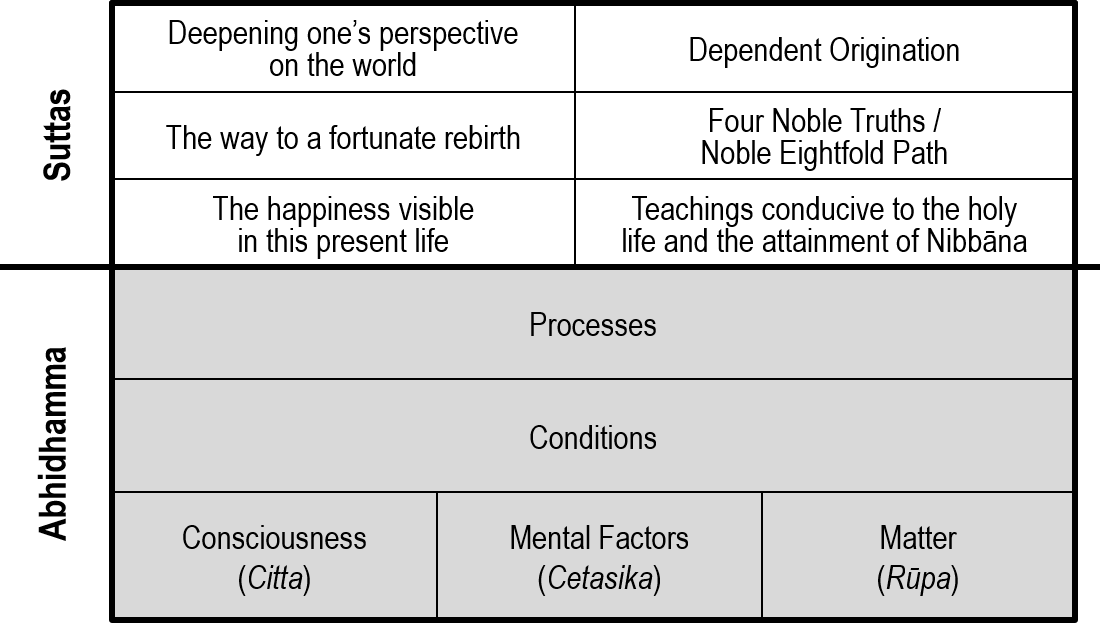
\includegraphics[width=0.6\linewidth]{./Diagrams/Block}
\caption{Block diagram showing topics in the Suttas and Abhidhamma.}
\label{fig:Block}
\end{figure}

The diagram in the middle of the handout shows the Suttas to be like the tip of the iceberg. The Suttas are what is visible. Below the water line, supporting all of the Suttas, is the unifying framework of the Abhidhamma.

Each Sutta is targeted at a specific audience to address a specific set of questions. To understand a specific Sutta, it is important to know the context in which it was given.\footnote{This contextual information, the background story for the Sutta, is often provided in the Commentary.} We can broadly classify the Suttas into two categories: Suttas delivered to laypeople\footnote{The structure of “The happiness visible in this present life/The way to a fortunate rebirth/Deepening one’s perspective on the world” is from Bhikkhu Bodhi’s book, “In the Buddha’s Words” (\url{http://www.pacificbuddha.org/wp-content/uploads/2014/01/In-the-Buddhas-Words.pdf}).} and Suttas delivered to monks.

\subsubsection*{Suttas given to laypeople}

For laypeople who were primarily interested in happiness visible in this present life, the Buddha gave simple, pragmatic teachings. In Buddhist countries, a popular topic for Dhamma talks is a Sutta\footnote{Sn 2.4: \url{http://en.wikipedia.org/wiki/Mangala_Sutta}\newline \url{http://www.accesstoinsight.org/tipitaka/kn/snp/snp.2.04.nara.html}} that lists 38 blessings, such as not associating with fools, generosity, respect and patience. Another popular Sutta\footnote{DN 31: \url{http://en.wikipedia.org/wiki/Sigalovada_Sutta}\newline \url{http://www.accesstoinsight.org/tipitaka/dn/dn.31.0.nara.html}} gives practical advice to a layperson regarding the reciprocal responsibilities between parents and children, teachers and students, etc. These topics are popular because they are immediately relevant to daily life and obviously lead to happiness in this present life.

Some laypeople were more spiritual and wanted to know the way to a fortunate rebirth. To address these concerns, there are Suttas that explain kamma\footnote{\url{http://en.wikipedia.org/wiki/Karma}} and ethics.\footnote{\url{http://en.wikipedia.org/wiki/Ethics}} Kamma and ethics will be discussed repeatedly during this course.

\pagebreak

There were also laypeople who were not ready to renounce but wanted to deepen their perspective on the world. Deepening one’s perspective on the world means “seeing things as they truly are,” with \textbf{Understanding}.\footnote{Words that are capitalized and in bold font are Mental Factors or \textit{rūpas}.} For many, the most challenging aspect of “seeing things as they truly are” is \textit{anattā}, or non-self. The ego constantly distorts perceptions, thoughts and opinions to put an artificial Self at the centre of its universe. This reminds me of a joke... a man goes into a book store looking for a book on Buddhist practice. He is directed to go to the “non-self” help section.

\subsubsection*{Suttas given to monks and nuns}

When talking to monks and nuns, the Buddha was addressing people who had already renounced and committed their lives to spiritual development.

The Buddha\footnote{SN 56.31: \url{http://www.accesstoinsight.org/tipitaka/sn/sn56/sn56.031.than.html}} once picked up a handful of leaves and asked the monks, “Which is more, the leaves in my hand or the leaves in the forest?” The Buddha compared what he had understood to the leaves in the forest while what he has taught he compared to the leaves in his hand. The Buddha then gave the criteria that he used to select what to teach: things conducive to the holy life and things leading to \textit{Nibbāna}.

In another Sutta,\footnote{MN 63: \url{http://www.accesstoinsight.org/tipitaka/mn/mn.063.than.html}} a monk asked the Buddha many theoretical questions such as “Is the cosmos eternal or not eternal, finite or infinite?” The Buddha told the monk that he was like a man wounded with a poisoned arrow who refused to have the arrow removed until he knew the name and height of the archer who shot the arrow, the type of bow that was used, the type of feathers on the arrow and many other details. The wounded man would die from the poison before finding all these answers. The Buddha explained that he did not teach things such as “Is the cosmos eternal or not eternal, finite or infinite” because these things are not conducive to the holy life and do not lead to \textit{Nibbāna}. The Buddha’s graphic analogy of removing a poisoned arrow reminds us of the urgency of our own spiritual development.

The Four Noble Truths\footnote{\url{http://en.wikipedia.org/wiki/Four_Noble_Truths}} are the principles of the Buddha’s teaching and the Noble Eightfold Path\footnote{\url{http://en.wikipedia.org/wiki/Noble_Eightfold_Path}} is the Buddha’s practical teaching on how to experience \textit{Nibbāna}. These are the essence of the Buddha’s teachings. Dependent Origination\footnote{\url{http://en.wikipedia.org/wiki/dependent_origination}} is the natural set of laws that cause beings to be bound to continuous rebirth. The topics of things conducive to the attainment of \textit{Nibbāna}, the Four Noble Truths, the Noble Eightfold Path and Dependent Origination are closely interrelated and are the central themes of many of the Suttas given to monks and nuns.

\pagebreak

\subsection*{Abhidhamma}

The third part of the \textit{Tipiṭaka} is the Abhidhamma.\footnote{\url{http://en.wikipedia.org/wiki/Abhidhamma_Pitaka}}

\begin{figure}[H]
\centering
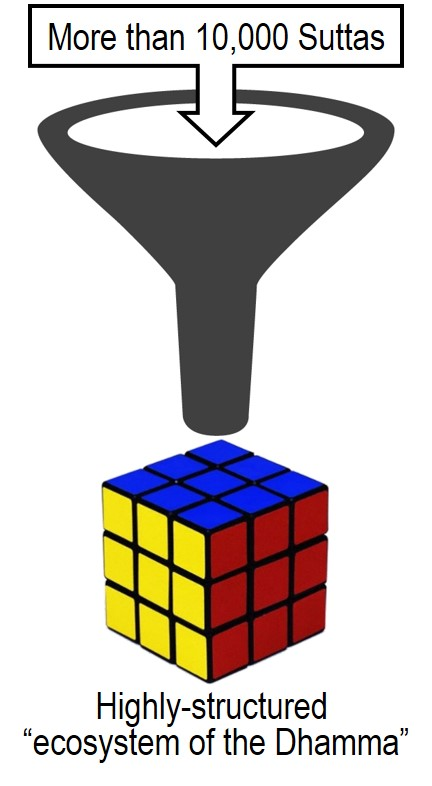
\includegraphics[width=0.25\linewidth]{./Diagrams/Funnel}
\caption{The Abhidhamma compresses more than 10,000 Suttas into a highly-structured framework or “ecosystem of the Dhamma” according to the Theravāda doctrine.}
\label{fig:Funnel}
\end{figure}

A monk\footnote{Correspondence with Jotinanda Bhikkhu.} recently wrote to me, “The Abhidhamma describes the underlying system upon which the Suttas are based. The Suttas were taught by the Buddha based on the mental disposition of the listeners and in a specific context. Because of this limitation, each Sutta can offer only a small window into the Buddha’s teaching; a window that gives one aspect of the Buddha’s teaching from one particular point of view. If we were to piece all these small windows together, strip away the context and repetitions, systematically analyze and place them into proper categories, draw out implications and elaborate them based on principles already found in the Suttas, we would eventually arrive at a complete picture of the entire `ecosystem’ of the Dhamma. This is the Abhidhamma view, unconstrained by any limitation\footnote{Limitation of scope to exclude things not related to the goal of liberation from suffering.} except the goal of liberation from suffering.”

In other words, the Abhidhamma is a framework or an ecosystem. It tries to consolidate content from all of the Suttas into a “big picture,” according to the Theravāda doctrine.

The Abhidhamma is more detailed and precise than the Suttas. For example, there are many Suttas which mention the five aggregates.\footnote{\url{http://en.wikipedia.org/wiki/Skandha}} In none of the Suttas is the discussion of the five aggregates more than half a page. The Abhidhamma\footnote{“The Book of Analysis” (\textit{Vibhaṅga}), pages 1--88.} includes an analysis of the five aggregates that is 88 pages long. So with all this detail, why is the Abhidhamma smaller than the Suttas? A lot of content in the Suttas relates to people, places, things and events. The Abhidhamma does not mention conventional topics such as people, places, things or events. It uses precise, technical terms – some taken from the Suttas and some created in the Abhidhamma – to create a comprehensive structure to open the door to a better understanding of the Suttas.

\subsubsection*{Ultimate Realities}

\begin{figure}[H]
\centering
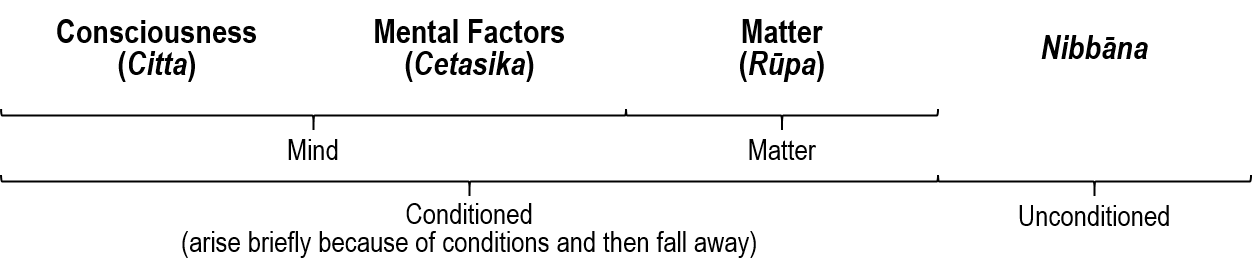
\includegraphics[width=0.9\linewidth]{./Diagrams/Realities}
\caption{The four Ultimate Realities: Consciousness, Mental Factors, Matter and \textit{Nibbāna}.}
\label{fig:Realities}
\end{figure}

The Buddha\footnote{DN 9: \url{http://www.accesstoinsight.org/tipitaka/dn/dn.09.0.than.html\#milk}} described names as “the world’s designations, the world’s expressions, the world’s ways of speaking, the world’s descriptions, with which the Buddha expresses himself but without grasping to them.” According to the Commentary, the Buddha is acknowledging two ways of communicating; in a conventional way using names and in a way using Ultimate Realities (the Abhidhamma communicates using Ultimate Realities).

The Abhidhamma\footnote{Ultimate Realities are not explicitly mentioned in the Abhidhamma \textit{Piṭaka}. The structure of “\textit{citta}, \textit{cetasika}, \textit{rūpa} and \textit{Nibbāna}” was introduced in the Abhidhammāvatāra (\url{http://en.wikipedia.org/wiki/Abhidhammavatara}), an Abhidhamma summary written around the time of Buddhaghosa. The Abhidhammāvatāra refers to this list as the “four most superior dhammas, the four shining truths.” \textit{Citta}, \textit{cetasika}, \textit{rūpa} and \textit{Nibbāna} were designated as Ultimate Realities (\textit{paramattha dhamma}) five centuries later in the Abhidhammattha Sangaha (about 1000 years ago).} classifies everything as either an Ultimate Reality\footnote{In the Abhidhamma, Ultimate Realities are used both from an ontological perspective (what is real?) and from an epistemological perspective (what is the object of right knowledge?).} or as a concept.\footnote{\url{http://en.wikipedia.org/wiki/Concept}} According to the Abhidhamma, the four Ultimate Realities are Consciousness (\textit{citta}), Mental Factors (\textit{cetasika}), Matter (\textit{rūpa}) and \textit{Nibbāna}. Consciousness and Mental Factors experience things; together, they are the mind (\textit{nāma}). The other two Ultimate Realities, Matter and \textit{Nibbāna}, are experienced by the mind. 

Consciousness, Mental Factors and Matter are conditioned; they arise based on conditions, exist for a brief instant and then cease to exist. It may seem that they are continuous but actually, many individual moments of Consciousness, Mental Factors and Matter arise in sequence. The Consciousness and Mental Factors that experience \textit{Nibbāna} are conditioned but \textit{Nibbāna} itself is “unconditioned;” \textit{Nibbāna} does not depend on conditions to come into existence.

\color{red}

What we call mind and body are temporary combinations of different Ultimate Realities, which arise because of conditions, and then fall away immediately. They are succeeded by new Ultimate Realities, which fall away again.

\color{black}

Wikipedia defines concept as “a generalization from experience or the result of a transformation of existing concepts.” “Person” is a concept, “house” is a concept and any form of label or idea is a concept. What is experienced through the senses is not a concept. In meditation, the idea of breathing is an example of a concept, but the temperature that is experienced, and the mind that experiences the temperature, are both examples of Ultimate Realities.

\color{red}

\textbf{Attachment} is an example of a Mental Factor, an Ultimate Reality. In Pāḷi, it is called \textit{lobha} and in other languages it has a different name. The name is a concept that changes whereas the underlying Ultimate Reality, that to which the name points, is universal.

\color{black}

\pagebreak

\subsubsection*{Consciousness (\textit{Citta})}

Let’s start with the block labelled “Consciousness,” or \textit{citta}\footnote{\url{http://en.wikipedia.org/wiki/Citta}} in Pāḷi.

The Suttas have multiple words for mind, such as “\textit{citta},” “\textit{mano},” “\textit{viññāṇa}” and “\textit{nāma}.” There is significant overlap in how these words are defined and used\footnote{The Suttas (SN 12.61: \url{http://www.accesstoinsight.org/tipitaka/sn/sn12/sn12.061.than.html}) explain we often take mind (\textit{citta}), intellect (\textit{mano}) and consciousness (\textit{viññāṇa}) as being Self.} in the Suttas.\footnote{\url{http://ahandfulofleaves.files.wordpress.com/2012/04/citta_mano_vinnana_a-psychosemantic-investigation_ucr_1965_johansson.pdf}} In the Abhidhamma, only the word “\textit{citta}” is used, and it refers to the Ultimate Reality of Consciousness. The Commentaries refer to a combination of Consciousness with its accompanying Mental Factors as a “Thought Moment.” The Pāḷi term for “Thought Moment” is “\textit{cittakkhaṇa},” which many writers shorten to “\textit{citta}.” In this course, I will consistently use the term “Thought Moment,” but if you encounter the word “\textit{citta}” in another text, you need to determine the meaning through the context.\footnote{\color {red} This term is challenging to translate.  In the Abhidhammattha Sangaha (most people’s first introduction to the Abhidhamma), the term “\textit{citta}” is used and many translators have left this word untranslated. I am not comfortable with using the term “\textit{citta}” to mean both the ultimate reality of consciousness and the combination of consciousness with Mental Factors. The original Abhidhamma texts use the term “\textit{dhamma}” for this combination and in the translation of these texts, the word “state” is used. Previously, I used the term “Mental State” for this combination of consciousness and Mental Factors, but this created confusion in people whose introduction to the Abhidhammattha Sangaha was Venerable Nārada’s translation, because Venerable Nārada used “Mental State” as a translation for “\textit{cetasika}”. In this Practical Abhidhamma course, I use the term “Thought Moment” for this combination of consciousness and Mental Factors, but you should not think of this as a measure of time. \color {black}}

According to the Commentaries, what is conventionally called the mind is actually a sequence of Thought Moments. Each Thought Moment arises based on conditions, performs its function and then falls away again. The talk on Consciousness will describe a map of the mind from the lowest states of mind such as hatred and lust, to the highest meditative states and attainments.

\subsubsection*{Mental Factors (\textit{Cetasika})\footnote{Details can be found in “Cetasikas” (see Footnote 2).}}

The next block is labelled “Mental Factors,” or \textit{cetasika}\footnote{\url{http://en.wikipedia.org/wiki/Mental_factors_(Buddhism)}} in Pāḷi.

The Mental Factors give the Thought Moment its individual character. Mental Factors include activities such as \textbf{Energy}, \textbf{Delusion}, \textbf{Attachment}, \textbf{Faith} and \textbf{Compassion}. 

Various terms found in the Suttas such as “craving,” “greed,” “covetousness” and “lust” are all represented in the Abhidhamma by a single Mental Factor; \textbf{Attachment}. The Abhidhamma focuses on the presence or absence of a Mental Factor in a Thought Moment, not on the intensity of the Mental Factor within the Thought Moment.

Mental Factors arise together and support each other. Understanding this relationship can provide practical insights. For example, understanding that \textbf{Delusion} is always working in the background whenever \textbf{Attachment} or \textbf{Aversion} arises, helps us to better understand the nature of \textbf{Attachment} and \textbf{Aversion}. The talk on Mental Factors will define each Mental Factor and explain which Thought Moments include which Mental Factors.

\subsubsection*{Matter (\textit{Rūpa})\footnote{Details can be found in “The Buddhist Teaching on Physical Phenomena” (see Footnote 2).}}

The next block is labelled “Matter,” or \textit{rūpa}\footnote{\url{http://en.wikipedia.org/wiki/Ruupa}} in Pāḷi.

How you describe something depends on what your objective is. For example, you may view a glass of water as something to drink when you are thirsty, a chef may view a glass of water as a cooking ingredient, and a scientist may view a glass of water as H$_{2}$O. All are correct. The suitable perspective depends on how water is to be used.

The Buddha’s teachings focus on spiritual development, so the Buddhist focuses on understanding how matter is experienced. For example, from a perspective of spiritual development, a glass of water has \textbf{Hardness}, \textbf{Heat}, \textbf{Odour} and \textbf{Taste}.

\subsubsection*{Conditions\footnote{Details can be found in “The Conditionality of Life” (see Footnote 2).}}

The block called Conditions sits on top of the three previous blocks: Consciousness, Mental Factors and Matter. Conditions explain how these ultimate realities can be related to each other. Everything arises because of multiple conditions. This can get very complex. During my talk on Conditions, I will focus on two conditions with the most practical applications\footnote{Other conditions will be identified in footnotes, but not described in the talks.} The talk will provide a practical understanding of kamma condition and of natural decisive support condition. 

\subsubsection*{Processes}

The final block in the diagram is Processes. This talk will explain seeing without a seer, thinking without a thinker, and the death and rebirth process\footnote{See Visuddhimagga XVI.90 (see footnote 2).}. Its focus will be on how an understanding of processes impacts practice. In my opinion, understanding the impact on practice is more important than the technical details.

\subsubsection*{Books of the Abhidhamma \textit{Piṭaka}}

I will now summarize the seven books of the Abhidhamma \textit{Piṭaka}. These do not form a cohesive set. Each book has a distinctive style and approach not found in the other books.\footnote{When reading the seven books of the Abhidhamma \textit{Piṭaka}, I get the impression that each book was written by different people at different times and each book was built up over time.}

The first book\footnote{\textit{Dhammasaṅgaṇī}, translated by the Pali Text Society as “A Buddhist Manual of Psychological Ethics.” Buddhaghosa’s Commentary, \textit{Atthasālinī}, has been translated by the Pali Text Society as “The Expositor.”} is a systematic listing of Thought Moments and Matter. The Mental Factors in each Thought Moment are listed and defined. 

The second book\footnote{\textit{Vibhaṅga}, translated by Pali Text Society as “The Book of Analysis.” Buddhaghosa’s Commentary, \textit{Sammohavinodanī}, has been translated by the Pali Text Society as “Dispeller of Delusion.”} is a set of essays. Many of the essays first analyze a topic using quotes from the Suttas, then analyze the same topic from the perspective of the Abhidhamma, and finally analyze the same topic in a “question and answer” section.

The third book\footnote{\textit{Dhātukathā}, translated by Pali Text Society as “Discourse on Elements.”} builds on the material in the first two books with a focus on aggregates, sense-bases and elements.\footnote{Aggregates (\textit{khandha}), sense-bases (\textit{āyatana}) and elements (\textit{dhātu}) are overlapping classifications from the Suttas.} For the items listed in the first book, the third book asks, “With how many aggregates is this item associated?” “With how many sense-bases is this item associated?” and “With how many elements is this item associated?” We will discuss aggregates, sense-bases and elements in later talks.

The fourth book\footnote{\textit{Puggalapaññatti}, translated by Pali Text Society as “Designation of Human Types.”} deals with classifications of persons, arranged numerically from one-fold to ten-fold. The presentation and much of the content mirrors the Suttas,\footnote{Specifically, the \textit{Aṅguttara Nikāya}.} leading some scholars to suggest that this is an early Abhidhamma text.

The fifth book\footnote{\textit{Kathāvatthu}, translated by Pali Text Society as “Points of Controversy.” Buddhaghosa’s Commentary has been translated by the Pali Text Society as “The Debates Commentary.”} is in the form of a debate on points of doctrine between the orthodox Theravāda view and opposing views. According to the Commentary, this book was composed at the conclusion of the Third Council, more than 200 years after the Buddha’s \textit{parinibbāna}.\footnote{The \textit{Kathāvatthu} quotes from the \textit{Dhammasaṅgaṇī}, \textit{Vibhaṅga} and \textit{Paṭṭhāna}, but makes no reference to the \textit{Dhātukathā} or \textit{Puggalapaññatti}. In addition, some of the schools that the \textit{Kathāvatthu} Commentary associates with certain heretical views in the \textit{Kathāvatthu} did not exist at the time of Aśoka. This suggests a gradual compilation of the Abhidhamma \textit{Piṭaka}.}

The sixth book\footnote{\textit{Yamaka}, not translated by Pali Text Society. The Pāḷi word \textit{yamaka} means “pairs.”} includes pairs of philosophical questions: Does X imply Y? and Does Y imply X?

The seventh book\footnote{\textit{Paṭṭhāna}, partially translated by Pali Text Society as “Conditional Relations.”} describes the conditions that relate Ultimate Realities to each other. It is called the “Great Book” because it is larger in size than the first six books combined.\footnote{The Pāḷi edition of the \textit{Paṭṭhāna} in Burmese script is 2500 pages long and the Pāḷi edition in Thai script is 6000 pages long; some (but not all) of the repetitive sections are expanded in the Thai version.}

\subsection*{The Abhidhamma as science and philosophy}

The Abhidhamma can be seen as the practical science of the mind – psychology without the psyche (no Self). It analyzes the mind into its component parts and classifies these parts into different categories.\footnote{For example, the \textit{Dhammasaṅgaṇī} lists more than 120 ways of classifying Thought Moments.} It gives us useful models and new ways of looking at the mind. The Abhidhamma has a precise set of specialized terminology used to describe different aspects of the mind. Analysis, classification, models, specialized terminology; sounds a lot like science, doesn’t it? Some writers try to draw parallels between Buddhism and modern science,\footnote{My bookshelf includes titles such as “Quantum Theory and Buddhism,” “Darwin’s Origin of Species according to the Buddha” (see \url{http://en.wikipedia.org/wiki/Buddhism_and_evolution}) and “Buddhist Theory of Causation and Einstein’s Theory of Relativity.”} but the objectives of the two are different; Buddhism is focused on spiritual development, so the similarities are superficial.

The Abhidhamma also covers aspects of philosophy. I know what you are thinking: “Philosophy is not practical.” But the Abhidhamma is not meant for abstract theorizing; the Abhidhamma can change your perspective on life. Ethics\footnote{\url{http://en.wikipedia.org/wiki/Ethics}} (what is morally right) and epistemology\footnote{\url{http://en.wikipedia.org/wiki/Epistemology}} (what is right knowledge) are useful aspects of philosophy described in the Abhidhamma. Another topic that is central to the Abhidhamma is what philosophers call “ontology;” \footnote{\url{http://en.wikipedia.org/wiki/Ontology}} the definition of what is real. This is practical because understanding what is real helps us to see things as they truly are and to recognize \textbf{Delusion} (mental blindness). Appreciating what is real and what is an illusion helps bring us back to the present moment. This is similar to what Eckhart Tolle calls “The Power of Now.” \footnote{\url{http://en.wikipedia.org/wiki/The_Power_of_Now}}

\subsubsection*{The Abhidhamma provides a simple model of how the mind works}

How can we develop an understanding of something as complicated as the mind? 

Science tackles the challenge of starting to understand complicated things by developing simple models.\footnote{\url{http://en.wikipedia.org/wiki/Scientific_modelling}} Let’s use weather as an example. Weather is far less complicated than the mind, but even today’s most powerful supercomputers are unable to predict the weather accurately. The first step that science took to understand weather was to develop simple models such as the Water Cycle.\footnote{\url{http://en.wikipedia.org/wiki/Water_cycle}} This model of condensation-precipitation-collection-evaporation is simple enough to be studied today by schoolchildren.

\begin{figure}[H]
\centering
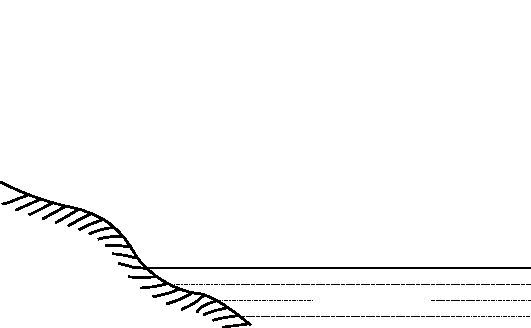
\includegraphics[width=0.85\linewidth]{./Diagrams/Rain}
\caption{The Water Cycle provides a simple model for a complex natural process.}
\label{fig:Rain}
\end{figure}

Because we have the simple model of the Water Cycle, we know that weather is a natural phenomenon even though we do not understand it very well.\footnote{\url{http://en.wikipedia.org/wiki/Weather_forecasting}} Because we know that weather is a natural phenomenon, we do not waste our time and resources performing rituals to try to please Weather Gods as our ancestors did. When people don’t understand things, their first reaction is to imagine a controlling entity such as a Weather God. The mind is complex and we don’t understand it, so we imagine a controlling entity called a Self and place this Self at the centre of our universe. The Abhidhamma provides a simple model of how the mind works.

Researchers\footnote{\url{http://www.andrewnewberg.com/books/why-god-wont-go-away-brain-science-the-biology-of-belief}} have used brain scanners\footnote{\url{http://en.wikipedia.org/wiki/Single-photon_emission_computed_tomography}} to examine the part of the brain that filters incoming data from the senses. This part of the brain also organizes the incoming sense data around an imagined Self. Normally, this part of the brain is extremely active. Researchers found that when a Buddhist is in deep meditation, the blood flow to this part of the brain is dramatically reduced. During these periods, when sense data is not filtered and not organized around an illusion of a Self, the Buddhist meditator experiences a “higher reality” which he describes as “oneness with the universe.” The same pattern can be seen in the brain of a Christian nun when she is deep in prayer. She describes the experience as “being in the presence of God.”

\begin{figure}[H]
\centering
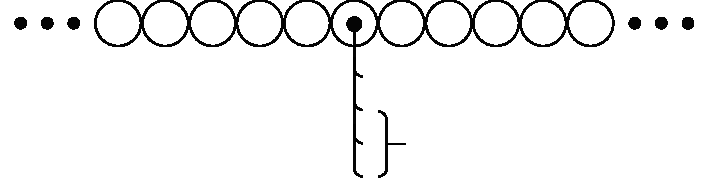
\includegraphics[width=1\linewidth]{./Diagrams/Model}
\caption{The Abhidhamma models the mind as a series of Thought Moments. Each Thought Moment arises, performs its function and then falls away. The falling away of one Thought Moment is a condition for the arising of the subsequent Thought Moment. Each Thought Moment includes Consciousness and a collection of Mental Factors.}
\label{fig:Model}
\end{figure}

The Suttas\footnote{MN 1: \url{http://www.accesstoinsight.org/tipitaka/mn/mn.001.than.html}} describe how the concept of Self is triggered by sense data, and during the talk on processes, we will explore the simple model from the Abhidhamma that explains how seeing happens without a seer, and how thinking happens without a thinker.

Just as the Water Cycle provides a simple model of how weather arises naturally without a controlling entity, the Abhidhamma provides a simple model of how sensing and thinking arise naturally without a Self. With this insight we will not waste time and energy on controlling the mind, and can instead focus on training the mind.

Training is building up natural habits in the mind. The mind is like a little puppy dog, it cannot be controlled but it can be trained. Buddhism teaches the gradual training of the mind;\footnote{\url{http://en.wikipedia.org/wiki/Gradual_training}\\MN 107: \url{http://www.accesstoinsight.org/tipitaka/mn/mn.107.horn.html}} precepts are rules of training.\footnote{The literal translation of \textit{sikkhāpada} is “factor (\textit{pada}) of training (\textit{sikkhā}).”} When we approach our spiritual development as a gradual training exercise, we then know that it requires lots of energy, lots of repetition, lots of patience and that it takes time. 

If you want to train yourself to play the piano well, you can’t just spend a few minutes on it from time to time. You have to commit to regular practice, energy, repetition, patience and time. The training associated with spiritual development requires a similar commitment (but the rewards are much greater than becoming a skilled pianist).

\begin{figure}[H]
\centering
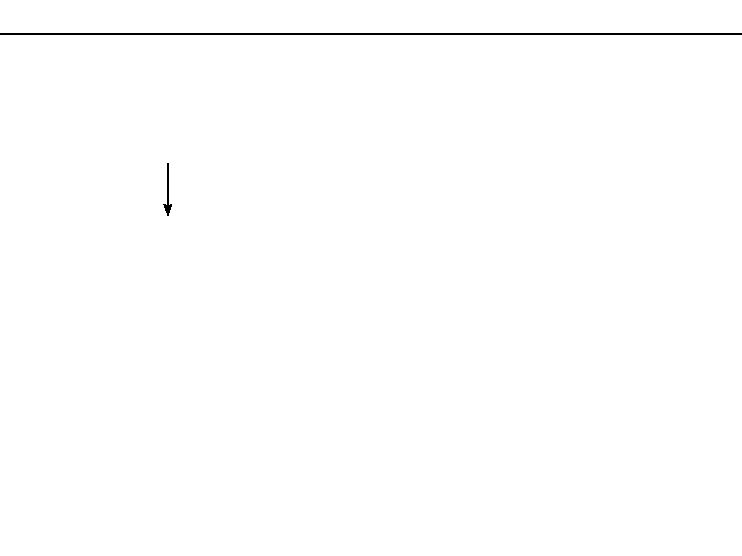
\includegraphics[width=1\linewidth]{./Diagrams/Libet}
\caption{Libet’s experiment challenges the concept of Free Will.}
\label{fig:Libet}
\end{figure}

Buddhism says there is deciding without a decider, and this challenges the notion of Free Will. Science is also starting to challenge the notion of Free Will. When Benjamin Libet\footnote{\url{http://en.wikipedia.org/wiki/Benjamin_Libet}} studied the electrical activity of the brain, he asked a person to push a button whenever they wanted. The data showed that it took about half a second for the electrical activity in the motor control centre of the brain to be transmitted to the finger pushing the button. Then Libet had the person indicate when they were aware of their intention to push the button. Libet expected the awareness of intention to come \textbf{before} the electrical activity but the data showed the opposite; the awareness of intention came \textbf{after} the electrical activity had already started. This means that the idea of a “Self that is making decisions” arises after decisions have already been made.\footnote{An interesting article: \url{http://www.nytimes.com/2007/01/02/science/02free.html?_r=0}}

“There is an I who decides” is an illusion, a justification and a rationalization that happens after a decision has already been made. Many find this disturbing because if my brain makes decisions before I am aware of the decisions being made, then how can I have Free Will? Is my fate determined? To Buddhists, the question of Free Will does not arise because there is no Self to have Free Will, so to use a Zen approach, you have to “un-ask the question.” A “Self with Free Will” is an illusion and a “Self whose fate is determined” is also an illusion. If Self is an illusion, if Free Will is an illusion, and if determinism is an illusion, how can there be moral responsibility? The answer is the natural law of kamma.

\subsection*{Application of Abhidhamma to spiritual development}

Here is a quote from a modern writer\footnote{This passage appears in both “The Abhidhamma in Practice” by Dr. N. K. G. Mendis (\url{http://www.bps.lk/olib/wh/wh322.pdf}) and “What Buddhists Believe” by Dr. K. Sri Dhammananda (\url{http://www.buddhanet.net/pdf_file/whatbelieve.pdf}).} that summarizes the application of Abhidhamma to spiritual development: “The question is raised whether the Abhidhamma is essential for Dhamma practice. The answer to this will depend on the individual who undertakes the practice. People vary in their levels of understanding, their temperaments and spiritual development. Ideally, all the different spiritual faculties should be harmonized, but some people are quite contented with devotional practices based on faith, while others are keen on developing penetrative insight. The Abhidhamma is most useful to those who want to understand the Dhamma in greater depth and detail. It aids the development of insight into the three characteristics of existence: impermanence, unsatisfactoriness, and non-self. It is useful not only for the periods devoted to formal meditation, but also during the rest of the day when we are engaged in various mundane chores. We derive great benefit from the study of the Abhidhamma when we experience absolute reality. In addition, a comprehensive knowledge of the Abhidhamma is useful for those engaged in teaching and explaining the Dhamma. In fact, the real meaning of the most important Buddhist terminologies such as Dhamma, \textit{Kamma}, \textit{Saṃsāra}, \textit{Sankhāra}, \textit{Paṭiccasamuppāda} and \textit{Nibbāna} cannot be understood without a knowledge of Abhidhamma.”

The Abhidhamma supports \textit{vipassanā} practice by providing the yogi and the teacher with a common vocabulary to describe experiences. However, Abhidhamma without meditation is theory without practice; it brings little if any benefit.\footnote{This story from the Commentary highlights the benefit of practice as compared to mere learning: \url{http://www.tipitaka.net/tipitaka/dhp/verseload.php?verse=019}} Theory without practice is like the spoon in a bowl of soup; the spoon is immersed in the soup but cannot experience the flavour. Meditation without Abhidhamma is practice without theory; it brings benefits, but in my opinion, progress may be slower because misunderstanding and \textbf{Doubt} may creep in. The best approach is meditation supported by an understanding of Abhidhamma. Mindfulness does not only arise when sitting on a cushion. We should try to integrate \textbf{Mindfulness} and \textbf{Understanding} into our daily activities.

Here is an analogy to illustrate the application of Abhidhamma. Imagine that you have never seen a beach before and then you see one from a distance. From a distance, the beach looks homogeneous. It takes energy to get there, but finally you are next to the beach. Now you can see that the beach is made of up an uncountable number of grains of sand. Next you get down on your knees and take out a powerful magnifying glass. At first, your hand is shaking so you cannot get the magnifying glass to focus. When your grip is steady, settled, unified and composed, you can focus the magnifying glass. You can see the details of each grain of sand. In this analogy, the grains of sand are the Ultimate Realities and the energy to move closer to the beach is the effort to look at Ultimate Realities. The mind is steady, settled, unified and composed.\footnote{The terms “Steady, settled, unified and composed” are used in the Suttas (such as MN 20:\newline \url{http://www.accesstoinsight.org/tipitaka/mn/mn.020.than.html}) to describe \textit{samatha}.} The details of each grain of sand are the characteristics of the Ultimate Realities.\footnote{Initially the specific characteristics of the Ultimate Reality will appear (i.e. \textbf{Attachment} is “sticky”), but eventually the general characteristics of \textit{anicca}, \textit{dukkha} and \textit{anattā} appear.}

\subsection*{Linkage to \textit{Satipaṭṭhāna} Sutta}

Please take a quick look through the \textit{Satipaṭṭhāna} Sutta. Bhikkhu Bodhi wrote:\footnote{From his translation of the \textit{Majjhima Nikāya}.} “This is one of the most important Suttas in the Pāḷi Canon, containing the most comprehensive statement of the direct way\footnote{“The direct way” is a translation of “\textit{ekāyana magga};” in the version of the \textit{Satipaṭṭhāna} Sutta provided, this phrase has been translated as “the only way” (see paragraph 2 and paragraph 74). This phrase should be interpreted as indicating directness of the path rather than exclusivity of the path.} to the attainment of the Buddhist goal.” Buddhists, particularly meditators,\footnote{The Commentary explains that the \textit{Satipaṭṭhāna} Sutta is intended for all meditators, not just monks.} need to be familiar with this Sutta. On first reading, this Sutta is not easy to understand. The detailed explanation of this Sutta given in the Commentary\footnote{See “The Way of Mindfulness” by Soma Thera: \url{http://www.accesstoinsight.org/lib/authors/soma/wayof.html}} is difficult to understand unless you have a foundation in Abhidhamma. The Abhidhamma is needed to understand the Commentaries and better appreciate the Theravāda interpretation of the Suttas.

Please look at paragraph 12 of the \textit{Satipaṭṭhāna} Sutta.\footnote{For some reason, the translator omitted a phrase from paragraph 12 regarding applying clear comprehension during defecating and urinating. In my opinion, this is an important phrase because it reinforces the idea that clear comprehension is to be applied during \textbf{all} daily activities.} You can see that \textbf{Mindfulness} and application of the Abhidhamma should be applied during all daily activities, not just during periods of formal meditation.

Many times during these talks, I will explain points from the \textit{Satipaṭṭhāna} Sutta using the Abhidhamma topic that we are discussing at that time. By the end of this Practical Abhidhamma course, you will have a better understanding of the \textit{Satipaṭṭhāna} Sutta, and of how the Abhidhamma helps you to a better understanding of the Suttas.

\subsection*{Summary of Key Points}

Here is a summary of key points from the Introduction:

\begin{itemize}

\item The Theravāda Buddhist canon consists of three collections:

\begin{itemize}

\item The Vinaya are the rules and procedures established by the Buddha to ensure harmonious interaction between monastics, and blameless interactions between monastics and laypeople.

\item The Suttas are the discourses delivered by the Buddha and his key disciples. Some Suttas were delivered to laypeople to address lay concerns. Other Suttas were delivered to help monastics with their spiritual development.

\item The Abhidhamma describes the underlying system upon which the Suttas are based. The Suttas were taught by the Buddha based on the mental disposition of the listeners and in a specific context. Because of this limitation, each Sutta can offer only a small window into the Buddha’s teaching; a window that gives one aspect of the Buddha’s teaching from one particular point of view. If we were to piece all these small windows together, strip away the context and repetitions, systematically analyze and place them into proper categories, draw out implications and elaborate them based on principles already found in the Suttas, we would eventually arrive at a complete picture of the entire “ecosystem” of the Dhamma. This is the Abhidhamma view, unconstrained by any limitation except the goal of liberation from suffering.

\end{itemize}

\item The Abhidhamma classifies everything as being either a concept or as one of the four Ultimate Realities: Consciousness, Mental Factors, \textit{Rūpa} (Matter) and \textit{Nibbāna}.

\item The Abhidhamma takes a scientific approach that analyzes the mind, categorizes Thought Moments, and provides a simple model of how the mind works; how there can be seeing without a seer and thinking without a thinker. In other words, how the mind can function without a Self.

\item The Abhidhamma supports \textit{vipassanā} practice by providing the yogi and the teacher with a common vocabulary to describe experiences.

\item The Abhidhamma is needed to understand the Commentaries and to better appreciate the Theravāda interpretation of the Suttas.

\end{itemize}

Finally, in my opinion, the most important thing to remember about this introduction is that the Abhidhamma is an important part of Theravāda Buddhism. The Abhidhamma gives us a better understanding of the Suttas by providing a framework that integrates all of the Buddha’s teachings.

\begin{center}
\textbf{\textit{This concludes the first talk.}} \\
\end{center}

\newpage

\subsection*{Questions \& Answers}

\question{How much does a layperson need to know about the Vinaya?}

The rules of the Vinaya apply to monastics, not to laypeople. Out of respect for monastics, laypeople should try to avoid situations where the monastic may break a Vinaya rule. The three most common Vinaya rules that may impact a layperson are 1) Monastics are not allowed to take solid food after solar noon\footnote{This Vinaya rule (and many others) do not apply when the monastic is sick.} 2) Monastics are not allowed to handle money, and 3) Monastics should not be alone with a member of the opposite sex.

Different monastics interpret these Vinaya rules in different ways. In the afternoon, some monastics will drink only water, while other monastics may consider cheese, chocolate or coffee to be allowable. Some monastics will touch money directly, some monastics may accept money in an envelope or on a tray, and some monastics have a lay attendant (called a \textit{kappiya}) who can accept money on their behalf.

As there is variation in practice, you should ask the monastic if you are unsure what is allowable. For a detailed explanation of the Vinaya from the perspective of a layperson, see \url{http://www.accesstoinsight.org/lib/authors/ariyesako/layguide.html}

\question{Since there are more than 10,000 Suttas, how should I approach such a large collection to get the most benefit?}

Bhikkhu Bodhi’s anthology of discourses titled “In the Buddha’s Words” (\url{http://www.pacificbuddha.org/wp-content/uploads/2014/01/In-the-Buddhas-Words.pdf}) is an excellent starting point. 

I highly recommend the “Access to Insight” website (\url{http://www.accesstoinsight.org/}), which has translations of more than 1000 Suttas. The website’s section, “Befriending the Suttas” (\url{http://www.accesstoinsight.org/befriending.html}) gives excellent advice. The website also includes an index of Suttas according to subject (\url{http://www.accesstoinsight.org/index-subject.html}) that makes it easy to find Suttas on a specific topic.

\question{My friend says that I should study the Suttas rather than spend time studying the Abhidhamma. How should I respond?}

In my opinion, it should not be “either the Suttas or the Abhidhamma.” In my opinion, you should study both the Suttas and the Abhidhamma. Each Sutta focuses on a specific message or set of messages. The Abhidhamma consolidates information from all of the Suttas into a coherent structure, so that deeper insights can be extracted when reading a specific Sutta. As you see in this course, there are many references to Suttas. The Suttas are the primary source of the Buddha’s teachings.

\color{red}

If you are going to study the Suttas seriously, then you will also want to refer to the Commentaries to better understand the more subtle points from the Suttas. The Commentary often uses the Abhidhamma to explain doctrine, so an understanding of Abhidhamma can be useful in understanding the Commentaries to the Suttas.

\color{black}

\pagebreak

\question{Some monks say that there are inconsistencies between the Abhidhamma and the Suttas. What is your opinion?}

The Abhidhamma represents a consolidation of the Suttas according to the orthodox Theravāda doctrine. Could there be other ways of consolidating the Suttas? Absolutely. Are there other ways of interpreting the Suttas that are not perfectly aligned with the orthodox Theravāda doctrine? Absolutely. In almost all cases, these apparent inconsistencies in no way impact the central tenets of Buddhism, so I do not consider them to be important.

I once met a senior monk with a PhD who said, “I have developed my own understanding of the Suttas based on my experience and I do not accept the Abhidhamma or the Commentaries.” After listening to him for a while, I replied respectfully, “Venerable Sir, your understanding may be correct, but I am unable to judge. If I follow your understanding, then I have only one source of information - you. If I stay with the interpretation of the Suttas according to the Abhidhamma and Commentaries, I have many sources of information, many books and many teachers.” \footnote{The Abhidhamma and the Commentaries have been subject to centuries of scrutiny.}

\color{red}

\question{Should I study the Abhidhamma before I start learning meditation? Do I need to study the Abhidhamma before I start learning meditation?}

In my opinion, you should start learning meditation before you study the Abhidhamma; just as one should time in the kitchen before studying a cookbook. Knowing some Abhidhamma is definitely not a prerequisite for a yogi, nor is it a prerequisite for a meditation teacher.

It is important to not allow the Abhidhamma to influence your meditation. When I enter the meditation hall, I leave the Abhidhamma at the door. I want to focus on what I am experiencing in the present moment and I don’t want the Abhidhamma to create expectations. Thinking about the practice is only thinking, it is not the practice. The practice is beyond words, beyond concepts, beyond the Abhidhamma. 

There is a story of a conversation between Ajahn Chah and an Abhidhamma teacher.\footnote{See section on “Buddhist Psychology” in \url{http://www.dhammatalks.net/Books2/Ajahn_Chah_A_Still_Forest_Pool.htm}} The teacher asked Ajahn Chah if he agreed that studying Abhidhamma was important. Ajahn Chah replied  “Yes, very important.” The teacher asked Ajahn Chah if his students learn Abhidhamma and he replied  “Oh yes, of course.” The teacher asked where they started, which books and which studies were best. Ajahn Chah replied, “Only here.” pointing to his heart, “Only here.”

In my opinion, students of Ajahn Chah can supplement the excellent teachings of Ajahn Chah with some practical understanding of Abhidhamma. 

\color{black}

\begin{figure}[H]
\centering
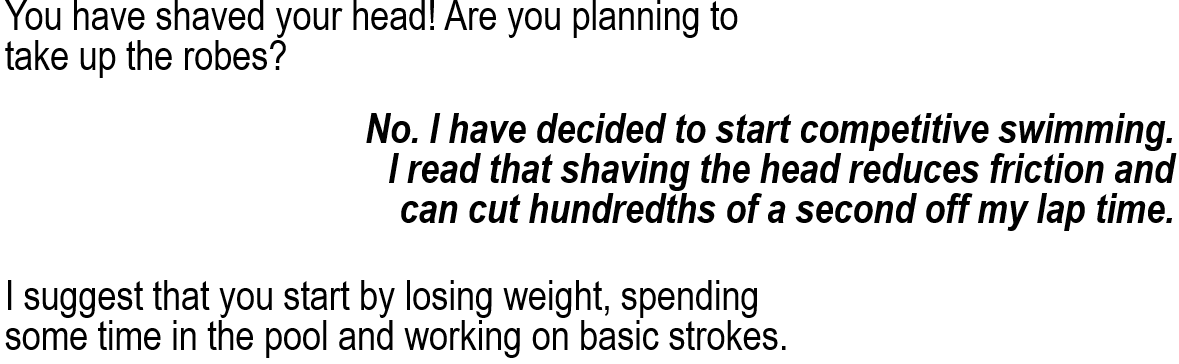
\includegraphics[width=0.7\linewidth]{./Diagrams/Swimming}
\caption{Some people obsess with minute details of the Abhidhamma and neglect basic practice.}
\label{fig:Swimming}
\end{figure}

This course focuses on the practical aspects of the Abhidhamma. I have omitted technical details that some people may find interesting but, in my opinion, are not practical. \color{red} Nevertheless, this “Practical Abhidhamma course” provides a solid foundation in the Abhidhamma should you wish to dive into more detail and study the Abhidhammattha Sangaha. My advice is to master the Abhidhammattha Sangaha before tackling the seven original Abhidhamma texts.

\color{black}

\question{Have you heard any jokes about Abhidhamma scholars?}

How many Abhidhamma scholars does it take to change a light bulb? There are 20W light bulbs, 40W light bulbs, 80W light bulbs, 100W… 200W… There are 6V light bulbs, 12V light bulbs, 120V light bulbs, 240V light bulbs… There are incandescent bulbs, fluorescent bulbs… There are clear light bulbs, pearled light bulbs, coloured light bulbs… There are screw-in light bulbs, bayonet light bulbs… There are 20W light bulbs that are 6V, there are 20W light bulbs that are 12V… 120V… 240V… There are 40W light bulbs that are 6V… 240V… 80W… 100W… 200W… There are 20W light bulbs that are 6V incandescent… There are 200W light bulbs that are 240V, florescent, coloured, and bayonet…\footnote{Some Abhidhamma scholars tend to avoid answering questions directly and instead recite long lists of categories.}
